\chapter{Implementation}
\label{chapter5}
\thispagestyle{plain}
Throughout this chapter we will go through the development phase of our proposed solution. In section \ref{design_patterns} we will see design patterns commonly used for development of web applications, as well as some examples from our application code in order to clarify the concepts. In section \ref{testing_validation} we will discuss methods that we use for testing and debugging our application.


%Later in section \ref{restful_controller} we implement a RESTFUL API in order to fetch data from our database, and in section <> we see how we can use the collected data in the front-end application via usage of RESTFUL Web service.
%Before we begin implementing our solution we need to discuss two dominant design patterns used in Web application development.

\section{Design patterns}
\label{design_patterns}
A design pattern is a general solution that addresses common software-design challenges. While not a finished design, you may think of a design pattern as a template or set of best practices. \cite{mvc_ref}
\subsection{MVC}
The model-view-controller (MVC) pattern is a software-design pattern used for creating data-driven web applications. 
In the design pattern of Model-View-Controller (MVC) the presentation of information (View) is separated from the information itself (Model) and the control or manipulation of the information (Controller).\cite{mvc_ref2} 

In an MVC architecture, most classes are either Models, Views or Controllers. The user interacts with Views, which display data held in Models. Those interactions are monitored by a Controller, which then responds to the interactions by updating the View and Model, as necessary. The View and the Model are generally unaware of each other because the Controller has the sole responsibility of directing updates. Generally speaking, Controllers will contain most of the application logic within an MVC application. Views ideally have little (if any) business logic. Models are primarily an interface to data and contain business logic to manage changes to said data.

The goal of MVC is to clearly define the responsibilities for each class in the application. Because every class has clearly defined responsibilities, they implicitly become decoupled from the larger environment. This makes the app easier to test and maintain, and its code more reusable, since it is not integrated with a specific presentation format. We choose MVC as design pattern of choice for our back-end application. Figure \ref{fig:mvc_pic_lbl} shows the adaptation of MVC architecture to the web application, using JAVA as a reference platform.

In order to use MVC pattern in our project we need to take a look at class diagram \ref{fig:uml_class_model}. As it is evident from diagram \ref{fig:uml_class_model}, we have five classes which we consider as our model objects.
A model is a simple POJO (Plain Old Java Object) class, as an example we model Guest class as:
\begin{verbatim}
->Guest.java
public class Guest {
  private int id;
  private String name;
  private String surName;
  private String passportNo;
  private String email;
  private String username;
  private String password;
  
  public String getId() {
    return id;
  }
  public void setId(int id) {
    this.id = id;
  }
  //... 
  // Above code is repeated for other fields for generating
  // getter and setter methods.
}
\end{verbatim}

Now that we have seen how a model class is created, we will see a Controller example. Example shown here is called \textit{RESTFUL} controller which we will see in section \ref{sec:restful_sec}. The controller receives HTTP requests  and responds to them, according to the defined path. This controller is in charge of API requests made by the front-end application. 
\label{restful_controller}
\begin{verbatim}
->Controller.java
@RequestMapping("/api")
@RestController
class ApiController {
  //... A repository containing the fetched data from database
  @Autowired
  private final GuestRepository repository;
  //... Mapping which connects a path to a method defined in 
  //... controller.
  @GetMapping("/guests")
  List<Guest> all() {
    return repository.findAll();
  }
}  
\end{verbatim}

The final piece of our MVC example is "View". We used Sencha ExtJS framework for our GUI application, however any plain HTML or JSP file is suitable for representing of a "View" to the client as long as an appropriate path and method for retrieving that view is defined in a Controller. 

\begin{figure} 
\centering
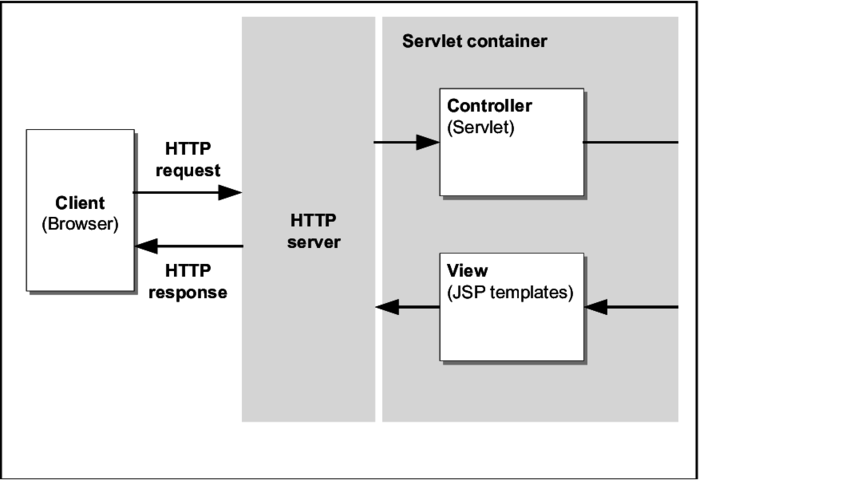
\includegraphics[width=12cm]{pictures/MVC_arch_pattern.png}
\caption{MVC Architectural design pattern}
Figure illustrating the MVC architecture applied to Web application. In this section we will see two design patterns for our back end and front end applications.
\label{fig:mvc_pic_lbl}
\end{figure}

\subsection{MVVM}
Another software-design pattern used in the development of our front-end application is Model View ViewModel (MVVM) design pattern. In MVVM, the View layer is concerned only about the graphical user interface, while the Model layer only about the business logic. All communication between them is realized by the ViewModel layer. \cite{mvvm_ref}

The key difference between MVC and MVVM is that MVVM features an abstraction of a View called the ViewModel. The ViewModel coordinates the changes between a Model’s data and the View's presentation of that data using a technique called “data binding”. The goal of MVVM is that the Model and framework perform as much work as possible, minimizing or eliminating application logic that directly manipulates the View.

In this section we go through each part of MVVM architectural pattern and see some examples:

\begin{itemize}
\item \textbf{Model}: This is the data for our application. A set of classes (called “Models”) defines the fields for their data (e.g. a Guest model with username and password fields). Models know how to persist themselves through the data package and can be linked to other models via associations.
\textbf{Store}: Models are normally used in conjunction with Stores to provide data for grids and other components. Models are also an ideal location for any data logic that you may need, such as validation, conversion, etc.
\item \textbf{View}: A View is any type of component that is visually represented. For instance, grids, trees and panels are all considered Views.
\item \textbf{Controller}: Controllers are used as a place to maintain the view's logic that makes the application work. This could entail rendering views, routing, instantiating Models, and any other sort of app logic.
\item \textbf{ViewModel}: The ViewModel is a class that manages data specific to the View. It allows interested components to bind to it and be updated whenever this data changes.
\end{itemize}

Figure \ref{fig:mvvm_pic_lbl} shows the adaptation of MVVM architecture for the Graphical User Interface (GUI) of our web application which lives inside the end user's browser.

Example code shown below represents a MVVM Model for our Booking class, defined in our front-end application.
\begin{verbatim}
-> Booking.js
// Definition of a Model class according to ExtJS framework
Ext.define('BookingApplication.model.Booking', {
//We need to extend the Model super class defined by ExtJS
extend: 'Ext.data.Model',
requires: ['Ext.data.proxy.JsonP'],
//We define model fields here
fields: [
{
    name: 'id',
    mapping: 'id' //-> Mapping our model fields to the Object 
// fields, coming from JSON response of back-end  
},
{
    name: 'startDate',
    mapping: 'startDate'
},
{
    name: 'endDate',
    mapping: 'endDate'
},
{
    name: 'numberOfPeople',
    mapping: 'numberOfPeople'
},
{
    name: 'paymentStatus',
    mapping: 'paymentStatus'
}],
proxy:
{
    type: 'ajax',
    url: '/api/bookings',
    reader: {
        type: 'json',
    }
}});
\end{verbatim}

As we can see in above code, "proxy" defines the type of call which is required to fill the model fields as well as the end point url on the back-end which responds to the call made by the object. The response which "reader" for this model expects is in from of a JSON message which we will discuss in section \ref{sec:json_sec}.

Now that we have seen how a model is defined in Sencha ExtJS framework, the next step is to define a ViewModel for our model. In the Below code section we can see that the Model for which we are defining a View Model must be referenced, there is also a \textit{Store} type of object which holds a collection of items of the type specified type. This store object is used inside the View to show the collection of objects to the user.

\begin{verbatim}
Ext.define('BookingApplication.view.main.BookingViewModel', {
  extend: 'Ext.app.ViewModel',
  alias: 'viewmodel.bookingviewmodel',
  requires: [
    'BookingApplication.model.Booking'
    ],
  stores: {
    bookings: {
      model:'BookingApplication.model.Booking',
      autoLoad: true
    }
  }
});
\end{verbatim}

We need a Grid object from the ExtJS framework libraries in order to show the collection of objects in the "Store" we have created. The Grid example shown below is later used inside our View.


\begin{verbatim}
Ext.define('BookingApplication.view.BookingGrid', 
{
    extend: 'Ext.grid.Grid',
    xtype: 'bookinggrid',
    cls: 'booking-grid',
    requires: [
        'Ext.grid.column.Column',
        'Ext.grid.cell.*'
    ],
    defaults: {
        height: 54
    },
    columns: [{
    text: 'id',
    dataIndex: 'id',
    flex: 1
    }, {
    text: 'startDate',
    dataIndex: 'startDate',
    flex: 1
    }, {
    text: 'endDate',
    dataIndex: 'endDate',
    flex: .5
    }, {
        text: 'numberOfPeople',
        dataIndex: 'numberOfPeople',
        flex: .5
    },{
        text: 'paymentStatus',
        dataIndex: 'paymentStatus',
        flex: .5
    }
]});
\end{verbatim}

Finally we proceed to insert the Grid we have created above, in our View.
As we can see in the code section below, we include a reference to our custom grid inside our View, we also have to reference the store object that we have created so that ExtJS framework loads the custom Grid with the store content.
\begin{verbatim}
Ext.define('BookingApplication.view.main.MainView', {
  extend: 'Ext.tab.Panel',
  xtype: 'mainview',
  requires: [
    'ModernTunes.view.main.BookingViewController',
    'ModernTunes.view.main.BookingViewModel',
  ],
  controller: 'bookingviewcontroller',
  
  viewModel: {
    type: "bookingviewmodel"
  },
  items: [
    {
        title: "Grid",
        xtype: 'tunesgrid',
        bind: {
          store: '{bookings}'
        } 
    }
  ]
});
\end{verbatim}

Now we have created our ViewModel and View. As the above code indicates, we also added BookingViewController. This controller handles interactions between the user and GUI application for this specific View.


\begin{figure} 
\centering
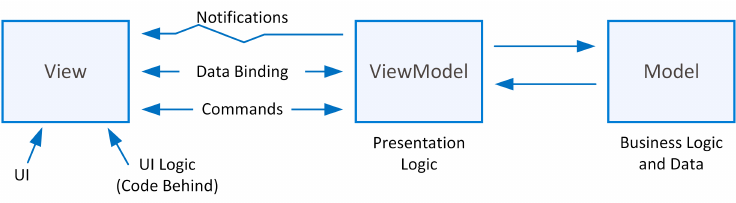
\includegraphics[width=12cm]{pictures/MVVM_arch_pattern.png}
\caption{MVVM Architectural design pattern}
Figure illustrating the MVVM architecture which is applied to the front-end application.
\label{fig:mvvm_pic_lbl}
\end{figure}




\section{RESTFUL Web Services}
\label{sec:restful_sec}
REpresentational State Transfer (REST) was originally introduced as an architectural style for building large-scale distributed hypermedia systems. REST leverages existing well known W3C/IETF standards (HTTP,XML,URI,MIME).\cite{rest_service}
The REST architectural style is based on four principles: \cite{rest_service}
\begin{itemize}
\item \textbf{Resource identification through URI}: A RESTFUL Web service exposes a set of resources which identify the targets of interaction with its clients. Resources are identified by URIs, which provide a global addressing space for resource and service discovery.
\item \textbf{Uniform interface}: Resources are manipulated using fixed set of four create, read, update, delete operations: PUT,GET,POST and DELETE. GET retrieves the current state of a resource in some representation. POST transfers a new state onto a resource.
\item \textbf{Self-descriptive messages}:
Resources are decoupled from their representation so that their content can be accessed in a variety of formats (e.g., HTML, XML, plain text, PDF, JPEG, etc.). Meta data about the resource is available and used for example control caching, detect transmission errors, negotiate appropriate representation format, and perform authentication or access control.
\item \textbf{Stateful interactions through hyperlinks}: 
Every interaction with a resource is stateless, i.e., request messages are self-contained. Stateful interactions are based on the concept of explicit state transfer. Several techniques exist to exchange state, e.g. URI rewriting, cookies, and hidden form fields. State can be embedded in response message to point to valid future states of the interactions. 
\end{itemize}

We use RESTFUL web services to create back-end APIs which respond to HTTP requests created by the front-end GUI application. These APIs allow us to create communications between the front-end client application and the back-end server application. An example request is provided below:
\begin{verbatim}
->An example request
GET localhost:8080/api/guests
\end{verbatim}
The server responds to this request by sending HTTP 200 (OK) status code which indicates that the request has been processed successfully on the server. In addition the response contains A JSON message corresponding to the requested source. We will discuss JSON in the next section.


%A RESTful API is an application program interface (API) that uses HTTP requests to GET, PUT, POST and DELETE data. An API for a website is code that allows two software programs to communicate with each other.

\section{JSON}
\label{sec:json_sec}
JSON (JavaScript Object Notation) is a lightweight data-interchange format. It is easy for humans to read and write. It is easy for machines to parse and generate. It is based on a subset of the JavaScript Programming Language Standard ECMA-262 3rd Edition - December 1999.\footnote{https://www.json.org/json-en.html}

JSON is used primarily to transmit data between our web application server and our front-end GUI application. Following on the example we made through this chapter, the JSON respond to the sample request made in section \ref{sec:restful_sec} is shown below.
\begin{verbatim}
->JSON response
 { 
 "id":"1", "name":"Max",
 "surName":"Wayne","passportNo":"T51617181",
 "email":"max.p@server.com","username":"maxwayne",
 "password":"0d0a96fa021ccd3fac05df1a584e3185" 
 } 
\end{verbatim}

\section{Testing \& Validation:}
\label{testing_validation}
In this section we will go through tools and methods used for testing our application. There are various testing methodologies which cover different aspects of either functional or non functional requirements.We will focus mainly on "Unit testing" and "System testing" due to the nature of the project. 

The goal of utilizing testing methodologies in development process is to make sure the software can successfully operate.
Testing methodologies can typically be broken down between functional and non-functional testing. Functional testing involves testing the application against the business requirements. It incorporates all test types designed to guarantee each part of a piece of software behaves as expected by using uses cases provided by the design team or business analyst.


\subsection{Unit Testing with JUnit}
Unit testing is the first level of testing and is often performed by the developers themselves. It is the process of ensuring individual components of a piece of software at the code level are functional and work as they were designed to. Developers in a test-driven environment will typically write and run the tests prior to the software or feature being passed over to the test team. Unit testing can be conducted manually, but automating the process will speed up delivery cycles and expand test coverage. Unit testing will also make debugging easier because finding issues earlier means they take less time to fix than if they were discovered later in the testing process. \footnote{https://smartbear.com/learn/automated-testing/software-testing-methodologies/}

\textit{JUnit} is a unit testing framework for the Java programming language. We can write unit tests manually or use already existing framework tools to generate automated tests.
The simple test shown below checks whether our "ApiController" is not \textit{null}.

\begin{verbatim}
package com.example.testingweb;
import static org.assertj.core.api.Assertions.assertThat;
import org.junit.jupiter.api.Test;
import org.springframework.beans.factory.annotation.Autowired;
import org.springframework.boot.test.context.SpringBootTest;

@SpringBootTest
public class ControllerTest {
	@Autowired
	private ApiController controller;

	@Test
	public void contexLoads() throws Exception {
		assertThat(controller).isNotNull();
	}
}    
\end{verbatim}

As mentioned above we can also write custom unit tests. Example shown below is a custom Unit test which checks whether "Guest" user has "PassportNo" field or not.

\begin{verbatim}
@ExtendWith(SpringExtension.class)
@SpringBootTest
class GuestRegisterTest {

  @Autowired
  private GuestService guestService;

  @Test
  void savedGuestHasPassportNumber() {
    Guest guest = new Guest("Max","Payne", "zaphod@mail.com");
    Guest savedGuest = guestService.registerGuest(guest);
    assertThat(savedGuest.getPassportNo()).isNotNull();
  }
}
\end{verbatim}


\subsection{System Test with LOG table}
In order to monitor the performance and availability of our application we need to implement a logging mechanism. We use the logging mechanism for troubleshooting issues and to make decisions about maintenance tasks.

Some of the required functionalities of a logging system are listed below:
\begin{itemize}
    \item Distinction between front-end and back-end application for logging errors/exceptions.
    \item Each application writes its own log using internal API, making sure that user requests are not blocked while logs are being written.
    \item The logging API collects log information produced by the application and sends it to the log database table.
\end{itemize}

We need to take into consideration that our application is using multi tier architecture, hence logs are separated by type of application. The decision of persisting logs into separate database tables or on a local log file located on the web application server depends on the level of autonomy and access given to developers by system administrator.

Another factor to consider is the number of concurrent requests to a certain database for accessing data (READ, WRITE operations) and the impact of log writing operations in case the log table is located on the same database server. We have decided on a log table located on the same server as our main database server, since the number of requests is not considerably large, later on this can be changed by adding a separate log server.

\textbf{LOG4J} is a reliable, fast and flexible logging framework (APIs) written in Java, which is distributed under the Apache Software License.

We use LOG4J to identify and collect exceptions occurring during an API call to our "ApiController". LOG4J allows  modification of layout of the log message, persistence in database and/or local file. In addition we can set \textit{level} of log, allowing for easy identification and categorization of events. A log request of level p in a logger with level q is enabled if p >= q. For the standard levels, we have \textit{ALL} < \textit{DEBUG} < \textit{INFO} < \textit{WARN} < \textit{ERROR} < \textit{FATAL} < \textit{OFF}. 
In order to log information into our database we need to create a LOG table. The SQL code below indicates the structure our LOG table.

\begin{verbatim}
CREATE TABLE LOGS
   (USER_ID VARCHAR(20)    NOT NULL,
    DATED   DATE           NOT NULL,
    LOGGER  VARCHAR(50)    NOT NULL,
    LEVEL   VARCHAR(10)    NOT NULL,
    MESSAGE VARCHAR(1000)  NOT NULL
   );    
\end{verbatim}

We also need to modify the LOG4J.properties file. This file contains settings which LOG4J uses to persist log data into the LOG table. 

\begin{verbatim}
<?xml version="1.0" encoding="UTF-8" ?>
<!DOCTYPE log4j:configuration SYSTEM "log4j.dtd">
<log4j:configuration>
<appender name="DB" class="org.apache.log4j.jdbc.JDBCAppender">
   <param name="url" value="jdbc:mysql://localhost/BOOKINGDB"/>
   <param name="driver" value="com.mysql.jdbc.Driver"/>
   <param name="user" value="root"/>
   <param name="password" value="****"/>
   <param name="sql" value="INSERT INTO LOGS 
   VALUES('%x','%d','%C','%p','%m')"/>
   <layout class="org.apache.log4j.PatternLayout">
   </layout>
</appender>
<logger name="log4j.rootLogger" additivity="false">
   <level value="DEBUG"/>
   <appender-ref ref="DB"/>
</logger>
</log4j:configuration>
\end{verbatim}

Now LOG4J is ready to persist log information. We can modify our "ApiController" by adding a logger which detects SQL Exception and persists it into our LOG table.

\begin{verbatim}
import org.apache.log4j.Logger;
import java.sql.*;
import java.io.*;
import java.util.*;
@RequestMapping("/api")
@RestController
public class ApiController{
   @Autowired
   private final GuestRepository;
   
   /* Get actual class name to be printed on */
   static Logger log = Logger.getLogger(ApiController.class.getName());
   
   @GetMapping("/guests")
   List<Guest> all() throws IOException,SQLException{
   try {
         return repository.findAll();
    } catch (SQLException e){
        log.debug("ERROR");
   }
}
\end{verbatim}

The same principles shown above is applied to the other methods inside "ApiController". We can set the log level shown in the above code to "DEBUG" or "INFO" in case we need to debug our code or retrieve a variable. The lines below show the actual result of execution of above code.

\begin{verbatim}
    mysql >  select * from LOGS;
+--------+------------+--------------+-------+---------+
| USER_ID| DATED      | LOGGER       | LEVEL | MESSAGE |
+--------+------------+--------------+-------+---------+
|  root  | 2019-05-13 | ApiController |ERROR |  ERROR  |
+--------+------------+--------------+-------+---------+
1 row in set (0.00 sec)
\end{verbatim}


\subsection{Debugger tools}
Now that we have seen the bug tracing via LOG table for our back-end application, we examine available tools to debug and test our front-end application. 

\textit{Secnha Inspector} is a debugging tool for troubleshooting and improving performance of Ext JS applications. Since \textit{Secnha Inspector} is a proprietary tool developed by Sencha we will not go through details of this tool in this report.

As an alternative we can debug our front end application, using developer tools found in modern browsers.

Image shown in \ref{fig:booking_detail_warning_pic} illustrates developer tools used to print some information on the debug console. 

There are two ways to debug JavaScript code.
\begin{enumerate}
    \item The first way, is to place console.log() in the code and see the value of the log, which will be printed in the console of the development tool.
    \item The second way is by using breakpoints in the development tool. Following is the process.
    \begin{itemize}
        \item Open the file in all the available scripts under script tag.
        \item Now place a breakpoint to the line you want to debug.
        \item Run the application in the browser.
        \item Now, whenever the code flow will reach this line, it will break the code and stay there until the user runs the code by keys F6 (go to the next line of the code), F7 (go inside the function) or F8 (go to the next breakpoint or run the code if there is no more breakpoints) based on the flow you want to debug.
        \item You can select the variable or the function you want to see the value of.
        \item You can use the console to check the value or to check some changes in the browser itself.
    \end{itemize}    
\end{enumerate}








%this will help us to identify and  critical level events from low level maintenance 



%Finally, our last concern is security, in case we need to store critically important logs which expose the vulnerabilities of our system. 



%One approach to a logging system is Bulk writing as opposed to single tuple writing. Bulk writing is used to optimize performance and minimize disruption of the application logic. This enables the platform to automatically generate detailed logging information and efficiently save it. 






